%!TEX root = ../dokumentation.tex

% Dokumentieren Sie diese Iterationen, Ihr Vorgehen und Ihre Fortschritte
% dazu in Form eines Protokolls mit 2-3 Seiten in Ihrem Entwurfsdokument.
% In der Iterationsphase ist es explizit erlaubt, sich mit anderen Teams
% auszutauschen, beispielsweise durch ein experimentelles Duell beider KIs.
% Nicht erlaubt ist es hingegen, Code von anderen zu kopieren. Bitte geben
% Sie an, mit welchen Teams sie zusammengearbeitet haben.

\chapter{Implementierung und Iteration}

Zu Beginn unseres Spielzuges wird innerhalb des AIPlayerControllers über jede Einheit auf dem Spielfeld gelooped. Hierbei wird für jede Einheit der MGPumDecisisonTreeManager aufgerufen. Innerhalb des Managers wird anhand des Namens der Einheit der jeweilige DecisionTree aufgerufen, um einen Zug zu ermitteln. Falls für die Einheit kein spezieller DecisionTree umgesetzt wurde, wird auf einen DefaultTree zurückgegriffen. Der ermittelte Zug wird dann zurückgegeben und ausgeführt.\\
Das Grundgerüst legt dabei die abstrakte Klasse MGPumDecisionTree. Dies enthält alle wichtigen Funktionen, wie beispielsweise das Ermitteln aller Angriffszüge und Bewegungen oder des kürzesten Weg zwischen zwei Feldern. Alle DecisionTrees werden später von diesem abgeleitet. 

\begin{figure}[H]
	\centering
	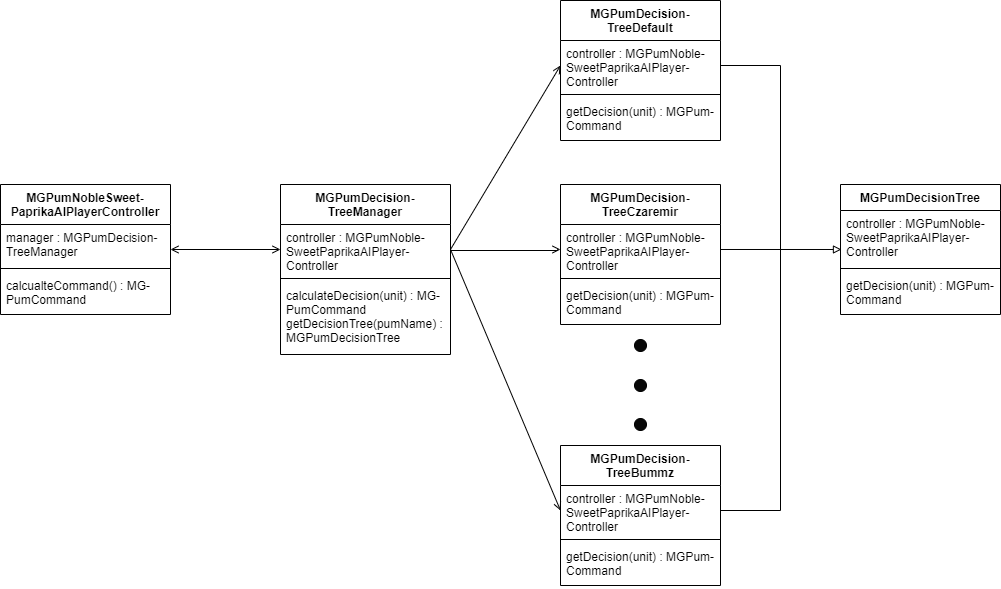
\includegraphics[width=1\linewidth]{klassendiagramm}
	\caption{Klassendiagramm der vollständigen Implementierung}
	\label{fig:klassendiagramm}
\end{figure}

% Beschreibung Angreifen --> DefaultTree
Das standardmäßige Angreifen erfolgt nach folgendem Ablauf. Im ersten Schritt werden mit Hilfe der Angriffsreichweite der Einheit alle möglichen Ziele und die Angriffszüge zu diesen ermittelt. Nun wird für jedes Ziel berechnet, ob dieses durch den Angriff stirbt. Es ergibt sich eine Liste aller besiegbaren Einheiten. Ist keine Einheit mit einem einzelnem Angriff besiegbar, wird für jeden möglichen Angriff innerhalb des Zuges untersucht, ob durch Kombinierung der Angriffe verschiedener Einheiten die gegnerische Einheit dennoch besiegt werden kann. Die resultierende Liste wird nun mit dem MGPumAttackCommandComparerKill sortiert. Wird keine zu tötende Einheit gefunden, wird die Liste aller angreifbaren Einheiten und der MGPumAttackCommandComparerAttack verwendet. Die im Spiel enthaltenen Einheit befinden sich hier in einer Hierarchiestruktur und bekommen eine Punktzahl, oder eine Funktion die diese berechnet, zugeordnet. Der Comparer vergleicht nun alle möglichen Ziele und sortiert diese nach dem besten Zug. Dieser kann dann ausgelesen und ausgeführt werden.

% Beschreibung allgemeines Laufen --> DefaultTree
Das standardmäßige Laufen erfolgt nach einem ähnlichen Ablauf. Im ersten Schritt werden mit Hilfe der Bewegungsreichweite der Einheit alle möglichen Felder zu denen sich die Einheit bewegen kann ermittelt. Um das bestmögliche Zielfeld zu ermitteln, wird ein MGPumMoveComparer verwendet. Dieser berechnet für jedes Feld eine Bewertung. Das Grundprinzip ist dabei genau eine gegnerische Einheit in Angriffsreichweite zu haben und von keiner Einheit angegriffen werden zu können. Hierzu wurde folgende Bewertungsfunktion eingesetzt: 

\begin{figure}[H]
	\centering
	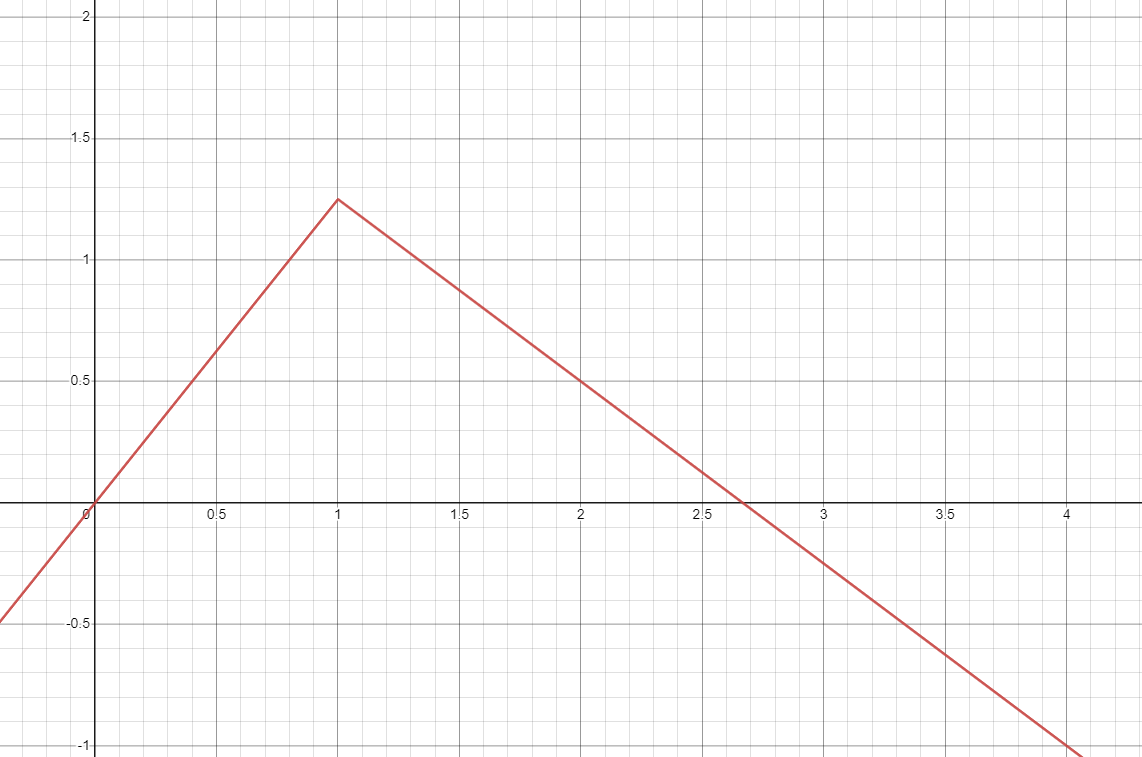
\includegraphics[width=0.8\linewidth]{bewertungsfunktion}
	\caption{Funktion zur Bewertung der Anzahl der möglichen Ziele}
	\label{fig:bewertungsfunktion}
\end{figure}

Diese wurde so angepasst, das ein Ziel die beste Bewertung erhält und zwei Ziele immer noch besser als kein Ziel zu bewerten ist, um ein zu passives Spielen zu verhindern. Von diesem Wert wird dann noch die Anzahl der Angreifer in Reichweite abgezogen. Auch diese Bewegungen werden anhand ihrer Bewertung sortiert und die beste davon ausgeführt. Falls die gegnerischen Einheiten zu weit entfernt sind und jede Bewegung gleich bewertet wird, werden Züge, welche sich in Richtung gegnerischer Einheiten bewegen, leicht präferiert.

\subsubsection{1. Iteration: Anpassung für Czaremir (How do you even pronounce that?)}

% Problem: alle Verhalten sich wie Default, manche Züge sehr aggressiv --> König intet
% passiver spielen
Nach einigen Spielbeobachtungen lässt sich erkennen, dass der Czaremir aufgrund des DefaultTrees oft zu aggressive Bewegungen durchführt, sich zu nah an Gegnern positioniert und deshalb unnötigen Schaden nimmt. Dementsprechend wird für ihn ein separater DecisionTree implementiert, welcher ihn passiver spielen lässt. Das bedeutet, dass Felder mit weniger Angreifer noch besser bewertet werden.

\subsubsection{2. Iteration: Anpassung für Range/Melee-Einheiten}

% grundlegender Tree zu passiv, eher Sniper Verhalten
% Ziel, Tank-Reihe bauen
% zurückhaltend nicht worth, Gegner greift allgemein auch immer an wenn er kann --> mehr worth die als Kanonenfutter zu benutzen
Nach weiteren Beobachtungen lässt sich erkennen, dass das allgemeine Verhalten zu passiv ist. Vor allem für Einheiten mit kleiner Angriffsreichweite lohnt es sich nicht sein Ziel auf 1 zu beschränken. Geht man davon aus, dass der Gegner ebenfalls versucht mit jeder möglichen Einheit anzugreifen, lässt sich allgemein sagen, dass das aggressivere spielen der Melee-Einheiten sinnvoller ist. Außerdem lässt sich so die im Konzept überlegte Blockade umsetzen, welche das Schützen von Range-Einheiten ermöglicht. Hierfür wird Anzahl der Angreifer zur Bewertung hinzugefügt statt abgezogen. Zudem wird die Positionierung bei eigenen Einheiten belohnt, um als Kanonenfutter Angriffe zu blocken.

\subsubsection{3. Iteration: Anpassung für Bummz}

% passiv is übel kacke, Fähigkeit als Vorteil nutzen --> weg von Mates, rein in Gegner
% Angriff auf Bummz: Berechnen ob worth wenn er stirbt auch rekursiv
Für die Bummz Einheit lässt sich schnell erkennen, dass eine passive Strategie sehr schlecht ist, da bei einer Explosion dem eigenen Team sehr viel Schaden zugefügt wird. Aus diesem Grund muss hier die Bewertung umgedreht werden. Felder sind dann gut bewertet, wenn wenig eigene und viele gegnerische Einheiten neben Bummz stehen. So kann seine Fähigkeit genutzt werden, um noch mehr Schaden am Gegner anzurichten. 

Auch im Sinne der Angriffsbewertung wurde die Fähigkeit von Bummz beachtet. In der Hierarchie der Einheiten erhält Bummz nun keinen festen Wert mehr sondern eine Funktion, welche den Angriff an der momentanen Stelle bewertet. Diese setzt sich zusammen aus dem verteilten Schaden an eigenen und gegnerischen Einheiten, wobei hier die Hierarchie der Einheiten und die mögliche rekursive Auslösung von anderen Bomben mit einbezogen wird. So erhält man je nach Feld und Spielstand eine individuelle Bewertung des Angriffes.

\subsubsection{4. Iteration: Anpassung für Draw}

% wenn nichts passiert zum Gegner
Nach 50 Zügen ohne Angriff erreicht das Spiel den Draw-Zustand. Ein Draw zeugt jedoch nicht von einer hohen Spielstärke und sollte vermieden werden. Deshalb soll zusätzlich zum DecisionTree nach 20 Zügen ohne Angriff das Zulaufen auf gegnerische Einheiten belohnt werden. Um sicherzustellen, dass Czaremir nicht unnötig an der Front steht, läuft dieser erst nach 30 Zügen Richtung Gegner.

\subsubsection{5. Iteration: Anpassung für Buff-Einheiten}

% ähnlich wie Default, weg von Gegner
% Zusatz: mehr Mates = besser
% kein spezieller Angriff
Buff-Einheiten haben eine spezielle Fähigkeit, welche ihre oder die Eigenschaften von Team-Mitgliedern verbessert. Um diese aktivieren zu können müssen diese direkt neben anderen Einheiten stehen. Der DecisionTree wird dementsprechend angepasst, dass ein Feld neben eigenen Einheiten eine bessere Bewertung erhält als Felder ohne. Im Falle von Haley und Buffy werden hierbei alle eigenen Einheiten mit einbezogen. Da Links nur eigene Links verstärken werden hierfür auch nur die andere Links betrachtet.

